\section{Introduction}
%\vspace{-3mm}
\label{sec:mohart_intro}


%\begin{figure}[b!]
%%    \vspace{-8mm}
%    \centering
%    \begin{subfigure}[c]{0.41\linewidth}
%        \centering
%        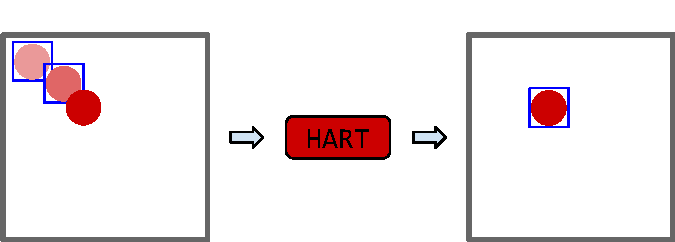
\includegraphics[width=\linewidth]{figures/MOHART/system_hart.pdf}
%%        \vspace{-5mm}
%        \caption{HART}
%    \end{subfigure}
%    \hspace{20mm}
%    \begin{subfigure}[c]{0.41\linewidth}
%        \centering
%        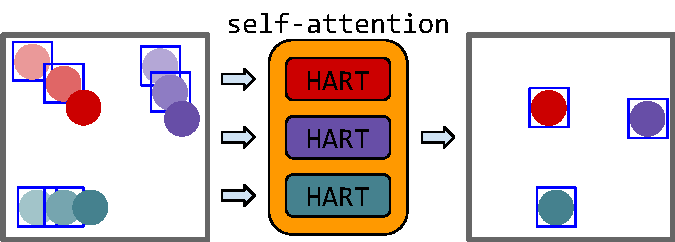
\includegraphics[width=\linewidth]{figures/MOHART/system_mohart.pdf}
%%        \vspace{-5mm}
%        \caption{MOHART}
%    \end{subfigure}
%%    \vspace{-2mm}
%    \caption{
%    Single-object tracking with \gls{HART} (left) and our extension to multi-object tracking (\gls{MOHART}, right). In our proposed framework, the different \gls{HART} trackers are connected via a relational reasoning module allowing for more robust tracking and more accurate future trajectory prediction.
%    % \vspace{-4mm}
%    }
%    \label{fig:teaser}
%\end{figure}


\begin{figure}[b!]
	   \vspace{-2mm}
	\centering
		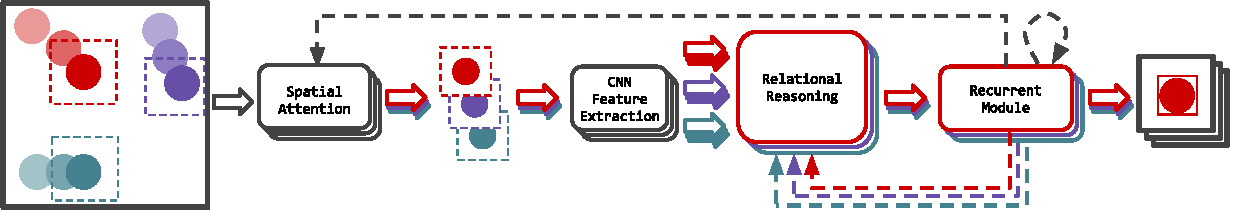
\includegraphics[width=\linewidth]{figures/MOHART/mohart_stacked.pdf}
	\vspace{-4mm}
	\caption{
		\Gls{MOHART}. A glimpse is extracted for each object using a (fully differentiable) spatial attention mechanism. These glimpses are further processed with a CNN and fed into a relational reasoning module. A recurrent module which iterates over time steps allows for capturing of complex motion patterns. It also outputs spatial attention parameters and a feature vector per object for the relational reasoning module. Dashed lines indicate temporal connections (from time step $t$ to $t+1$). The entire pipeline operates in parallel for the different objects, only the relational reasoning module allows for exchange of information between tracking states of each object. \gls{MOHART} is an extension of \acrshort{HART} (a single-object tracker), which features the same pipeline without the relational reasoning module.
	}
	\label{fig:teaser}
\end{figure}

Real-world environments can be rich and contain countless types of interacting objects.
Intelligent autonomous agents need to understand both the objects and interactions between them if they are to operate in those environments.
This motivates the need for \emph{class-agnostic} algorithms for tracking multiple objects---a capability that is not supported by the popular tracking-by-detection paradigm.
% In tracking-by-detection, static video frames are first analysed by an object detector,\eg a pre-trained deep \gls{CNN} such as \textsc{yolo} \citep{Redmon15}, and then the detected objects are linked across frames. 
In tracking-by-detection, objects are detected in each frame independently,\eg by a pre-trained deep \gls{CNN} such as \textsc{yolo} \citep{Redmon15}, and then linked across frames. 
%
Algorithms from this family can achieve high accuracy, provided sufficient labelled data to train the object detector, and given that all encountered objects can be associated with known classes, but fail when faced with objects from previously unseen categories.
%

\Gls{HART} is a recently-proposed, alternative method for single-object tracking (\textsc{sot}), which can track arbitrary objects indicated by the user (see \Cref{ch:hart}).
%
This is done by providing an initial bounding-box, which may be placed over any part of the image, regardless of whether it contains an object or what class the object is.
% 
\Gls{HART} efficiently processes just the relevant part of an image using spatial attention; it also integrates object detection, feature extraction, and motion modelling into one network, which is trained fully end-to-end.
Contrary to tracking-by-detection, where only one video frame is typically processed at any given time to generate bounding box proposals, end-to-end learning in \gls{HART} allows for discovering complex visual and spatio-temporal patterns in videos, which is conducive to inferring what an object is and how it moves.
%

In the original formulation, \gls{HART} is limited to the single-object modality---as are other existing end-to-end trackers \citep{Kahou2015ratm,Danesh2019deep,Gordon2018re3}.
%
In this work, we present \gls{MOHART}, a class-agnostic tracker with complex relational reasoning capabilities provided by a multi-headed self-attention module \citep{Vaswani17,Lee2019set}. 
\Gls{MOHART} infers the latent state of every tracked object in parallel, and uses self-attention to inform per-object states about other tracked objects.
This helps to avoid performance loss under self-occlusions of tracked objects or strong camera motion.
Moreover, since the model is trained end-to-end, it is able to learn how to manage faulty or missing sensor inputs. See \cref{fig:teaser} for a high-level illustration of \gls{MOHART}.

In order to track objects, \gls{MOHART} estimates their states, which can be naturally used to predict future trajectories over short temporal horizons, which is especially useful for planning in the context of autonomous agents.
\gls{MOHART} can be trained simultaneously for object tracking and trajectory prediction at the same time, thereby increasing statistical efficiency of learning. 
In contrast to prior art, where trajectory prediction and object tracking are usually addressed as separate problems with unrelated solutions, our work show trajectory prediction and object tracking are best addressed jointly.

\Cref{sec:mohart_related} describes prior art in tracking-by-detection, end-to-end tracking and predestrian trajectory prediction. In \Cref{sec:mohart_method}, we describe our approach, which uses a permutation-invariant self-attention module to enable tracking multiple objects end-to-end with relational reasoning. 
\Cref{sec:experiment_toy} contrasts our approach with multi-object trackers which do not explicitly enforce permutation invariance but have the capacity to learn it, simpler permutation-invariant architectures, as well as multiple single-object trackers running in parallel.
We show that multi-headed self-attention significantly outperforms other approaches. 
Finally, in \Cref{sec:experiment_real}, we apply \gls{MOHART} to real world datasets and show that permutation-invariant relational reasoning leads to consistent performance improvement compared to \gls{HART} both in tracking and trajectory prediction.




%%%%%%%%%%%%%%%%%%%% 0925 - some ideas
% The majority of contemporary object-tracking approaches used in autonomous vehicles do not model interactions between objects. This contrasts with the fact that object paths are not independent. For example, a cyclist might abruptly deviate from a previously planned trajectory in order to avoid colliding with a car. To fully leverage the potential of relational reasoning for real-world applications, like multi-object tracking, we propose that a relational-reasoning module ought to access both appearance features and previous motions of all objects involved. 
% % To explore these ideas, we introduce a multi-object version of \gls{HART} \citep{Kosiorek17} which we refer to as \gls{MOHART}. 
% In order to provide the relational reasoning module with the maximum richness of appearance and motion information, we built on an end-to-end single object tracker, \gls{HART} \citep{Kosiorek17}, and extent it to multi-object tracking (\gls{MOHART}) with relational reasoning.

% End-to-end object trackers comprise a newly developed, less explored area of research and break with the popular tracking-by-detection paradigm. In tracking-by-detection, static video frames are first analysed by an object detector,\eg a pre-trained deep \gls{CNN} such as \textsc{yolo} \citep{Redmon15}, and then the detected objects are linked across frames. 

% Importantly, the entire \gls{MOHART} system, including the way it models interactions and relations between objects, is class-agnostic and is trained end-to-end (\Cref{fig:teaser}). While \gls{HART} only tracks a single object, \gls{MOHART} connects multiple \gls{HART} modules, performing relational reasoning using a self-attention mechanism. Concretely, the relational-reasoning module receives a list of feature vectors, one per object, as input. This part of the problem is permutation invariant, as the list-order of object representations carries no meaning for the task at hand. 


% In Section 3 we describe our approach, using self-attention with explicit permutation invariance to enable tracking multiple objects end-to-end with relational reasoning independent of the order in which they are detected. 
% In Section 4 we compare our approach to multiple single object trackers running in parallel, multi-object trackers which do not explicitly enforce permutation invariance but have the capacity to learn it, as well as simpler permutation invariant architectures. We show that multi-headed self-attention significantly outperforms the other approaches. Finally, in \Cref{sec:experiment_real}, we apply \gls{MOHART} to real world datasets and show that permutation invariant relational reasoning leads to consistent performance improvement compared to \gls{HART} both in tracking and trajectory prediction.
%%%%%%%%%%%%%%%%%%%% end of 0925 - some ideas


%%%%%%%%%%%%%%%%%%%% Version 0924
% The majority of contemporary object-tracking approaches used in autonomous vehicles do not model interactions between objects. This contrasts with the fact that object paths are not independent. For example, a cyclist might abruptly deviate from a previously planned trajectory in order to avoid colliding with a car. To fully leverage the potential of relational reasoning for real-world applications, like multi-object tracking, we propose that a relational-reasoning module ought to access both appearance features and previous motions of all objects involved. 
% % To explore these ideas, we introduce a multi-object version of \gls{HART} \citep{Kosiorek17} which we refer to as \gls{MOHART}. 
% In order to provide the relational reasoning module with the maximum richness of appearance and motion information, we built on an end-to-end single object tracker, \gls{HART} \citep{Kosiorek17}, and extent it to multi-object tracking (\gls{MOHART}) with relational reasoning.


% Importantly, the entire \gls{MOHART} system, including the way it models interactions and relations between objects, is class-agnostic and is trained end-to-end (\Cref{fig:teaser}). While \gls{HART} only tracks a single object, \gls{MOHART} connects multiple \gls{HART} modules, performing relational reasoning using a self-attention mechanism. Concretely, the relational-reasoning module receives a list of feature vectors, one per object, as input. This part of the problem is permutation invariant, as the list-order of object representations carries no meaning for the task at hand. 


% The paper is organised as follows. In \Cref{sec:method}, we describe a set of methods, including self-attention, for modelling relational reasoning. In \Cref{sec:experiment_toy}, we show that processing information in a non permutation invariant manner shows no performance improvement compared to single object tracking (i.e.~no relational reasoning), despite being theoretically capable of \emph{learning} permutation invariance and having more capacity. In this setting, we demonstrate that the alternative DeepSets architecture \citep{Zaheer2017,Komiske2019,Qi2017,Qi2017a,Wagstaff2019} is inferior to multi-headed self-attention \citep{Vaswani17,Lee2019settransformer}, despite the DeepSets architecture in theory allowing for universal approximation of all permutation invariant functions \citep{Zaheer2017,Wagstaff2019}. Finally, in \Cref{sec:experiment_real}, we apply \gls{MOHART} to real world datasets and show that permutation invariant relational reasoning leads to consistent performance improvement compared to \gls{HART}.

% In Section 3 we describe our approach, using self-attention with explicit permutation invariance to enable tracking multiple objects end-to-end with relational reasoning independent of the order in which they are detected. 
% In Section 4 we compare our approach to multiple single object trackers running in parallel, multi-object trackers which do not explicitly enforce permutation invariance but have the capacity to learn it, as well as simpler permutation invariant architectures. We show that multi-headed self-attention significantly outperforms the other approaches. Finally, in \Cref{sec:experiment_real}, we apply \gls{MOHART} to real world datasets and show that permutation invariant relational reasoning leads to consistent performance improvement compared to \gls{HART} both in tracking and trajectory prediction.
%%%%%%%%%%%%%%%%%%%% end of Version 0924


% Finally, in Section 5 we apply MOHART to real-world datasets exemplifying the important role that permutation invariant multi-object trackers will play in multi-object tracking and trajectory prediction applications in the future.


%These feature vectors contain information about appearance and previous motion. The output of the relational reasoning module, one per tracked object, is then fed into an LSTM and 

%
%Autonomous vehicles need to operate in rich environments that contain a large variety of interacting object. 
%%
%This variety motivates the need for \emph{class-agnostic} object trackers, which break with the popular tracking-by-detection paradigm \citep{Zhang2008,Milan2014,bae2017confidence, keuper2018motion}. 
%%
%In tracking-by-detection, static video frames are first analysed by an object detector,\eg a pre-trained deep \gls{CNN} such as \textsc{yolo} \citep{Redmon15}, and then the detected objects are linked across frames. 
%%
%Algorithms from this family can achieve high accuracy, provided sufficient labelled data to train the object detector, and given that all encountered objects can be associated with known classes. 
%%
%
%\Gls{HART} is a recently proposed alternative for single-object tracking (\textsc{sot}), where an arbitrary object can be tracked from an initial video frame \citep{Kosiorek17}.
%%
%Since the initial bounding-box is user-provided and may be placed over any part of the image, regardless of whether it corresponds to an object and its class, \gls{HART} can track arbitrary objects.
%% 
%\Gls{HART} efficiently processes just the relevant part of an image using spatial attention; it also integrates object detection, feature extraction, and motion modelling into one network, which is trained fully end-to-end.
%Contrary to tracking-by-detection, where only one video frame is typically processed at any given time to generate bounding box proposals, end-to-end learning in \gls{HART} allows discovering complex visual and spatio-temporal patterns in videos, which is conducive to inferring what an object is and how it moves.
%%
%
%In the original formulation, \gls{HART} is limited to the single-object modality---as are other existing end-to-end trackers \citep{Kahou15,Danesh19,Gordon2018}.
%%
%In this work, we present \gls{MOHART}, a class-agnostic tracker with complex relational reasoning capabilities provided by a multi-headed self-attention module \citep{Vaswani17,Lee2019settransformer}. 
%\Gls{MOHART} infers the latent state of every tracked object in parallel, and uses self-attention to inform per-object states about other tracked objects.
%This helps to avoid performance loss under self-occlusions of tracked objects or strong ego-motion.
%Moreover, since the model is trained end-to-end, it is able to learn how to manage faulty or missing sensor inputs.
%It can also use the inferred objects' states to predict their future trajectories, which depend on interactions between different objects. See \cref{fig:teaser} for a high-level illustration of \gls{HART} and \gls{MOHART}.
%
%After describing related work in \Cref{sec:related} and the methodology in \cref{sec:method}, we employ the algorithm on toy domains to validate its efficacy in \Cref{sec:experiment_toy}. By controlling the stochasticity of toy environments, we show that single-object tracking is sufficient in some cases, even those featuring strong long-range interactions, while it may fail in other cases.
%This may hint at a similar phenomenon in the real world: tracking objects or predicting their future motion independently may be possible in most (but not all) cases, while solving the remaining corner cases might require taking interactions between objects into account.
%It is these corner cases that motivate our work.
%In \Cref{sec:experiment_real}, we test \gls{MOHART} on three real world datasets (MOTChallenge \citep{MOT16}, UA-DETRAC \citep{Wen15}, Stanford Drone dataset \citep{DroneDataset}) and show that relational reasoning between objects is most important on the MOTChallenge dataset. We hypothesise that this is due to its richness in ego-motion, occlusions and crowded scenes---a result supported by our ablation study. Furthermore, we show that \gls{MOHART} is able to gracefully handle missing sensory inputs---without any architectural changes. In this case, it falls back on its internal motion model, which also allows for accurate prediction of object locations multiple time steps into the future, learned in a data-driven manner.


